\documentclass[11pt, letterpaper]{article}
\usepackage[margin=0.5in]{geometry}
\usepackage{graphicx}

\begin{document}

\title{Comparison of Performance Across Suffix Tries, Trees, and Arrays}
\author{Jason Hunter}
\maketitle

\section{Introduction}
In my analysis, I implemented and ran comparisons on several suffix data structures - 
specifically suffix tries, suffix trees, and suffix arrays. 
I then compared the performance of these data structures in terms of runtime and memory usage, with
the goal of determining which data structure is the best choice for sequence processing tasks relevent to bioinformatics.
I developed methods for constructing these structures and querying them. In my search for more efficient data structures, I came across
Ukonnen's algorithm, which is a linear time algorithm for constructing suffix trees, and subsequently suffix arrays as well.
I used this algorithm to construct suffix trees and suffix arrays, and compared their performance to that of suffix tries,
as well as to the basic suffix tree and suffix array construction approaches. 
The experiments I ran showed that suffix arrays are the most efficient data structure in terms of runtime and memory usage,
particularly at scale when the size of the input sequence is large. This is even more pronounced when the suffix array is constructed using Ukonnen's algorithm.
Suffix tries were very memory intensive, and could only be used for small input sequences. Suffix trees were more memory efficient than suffix tries, but still
used more memory than suffix arrays, especially when using the naive construction approach. Ukonnen's algorithm was able to construct suffix trees and suffix arrays
in close to linear time, which was a significant improvement over the naive construction approach. Ultimately, I found that the suffix array constructed using Ukonnen's algorithm
was the only data structure that could handle large input sequences larger than 100,000 efficiently, and is the best choice for sequence processing tasks in bioinformatics.



\section{Results}
I created a benchmark suite to compare the performance of suffix tries, suffix trees, and suffix arrays.
It builds and queries each structure using a variety of input sequences, and records the time and memory usage for each operation.
The following graphs show the results of these benchmarks.

\subsection{Runtime Comparison} 

\begin{figure}[ht]
  \centering
  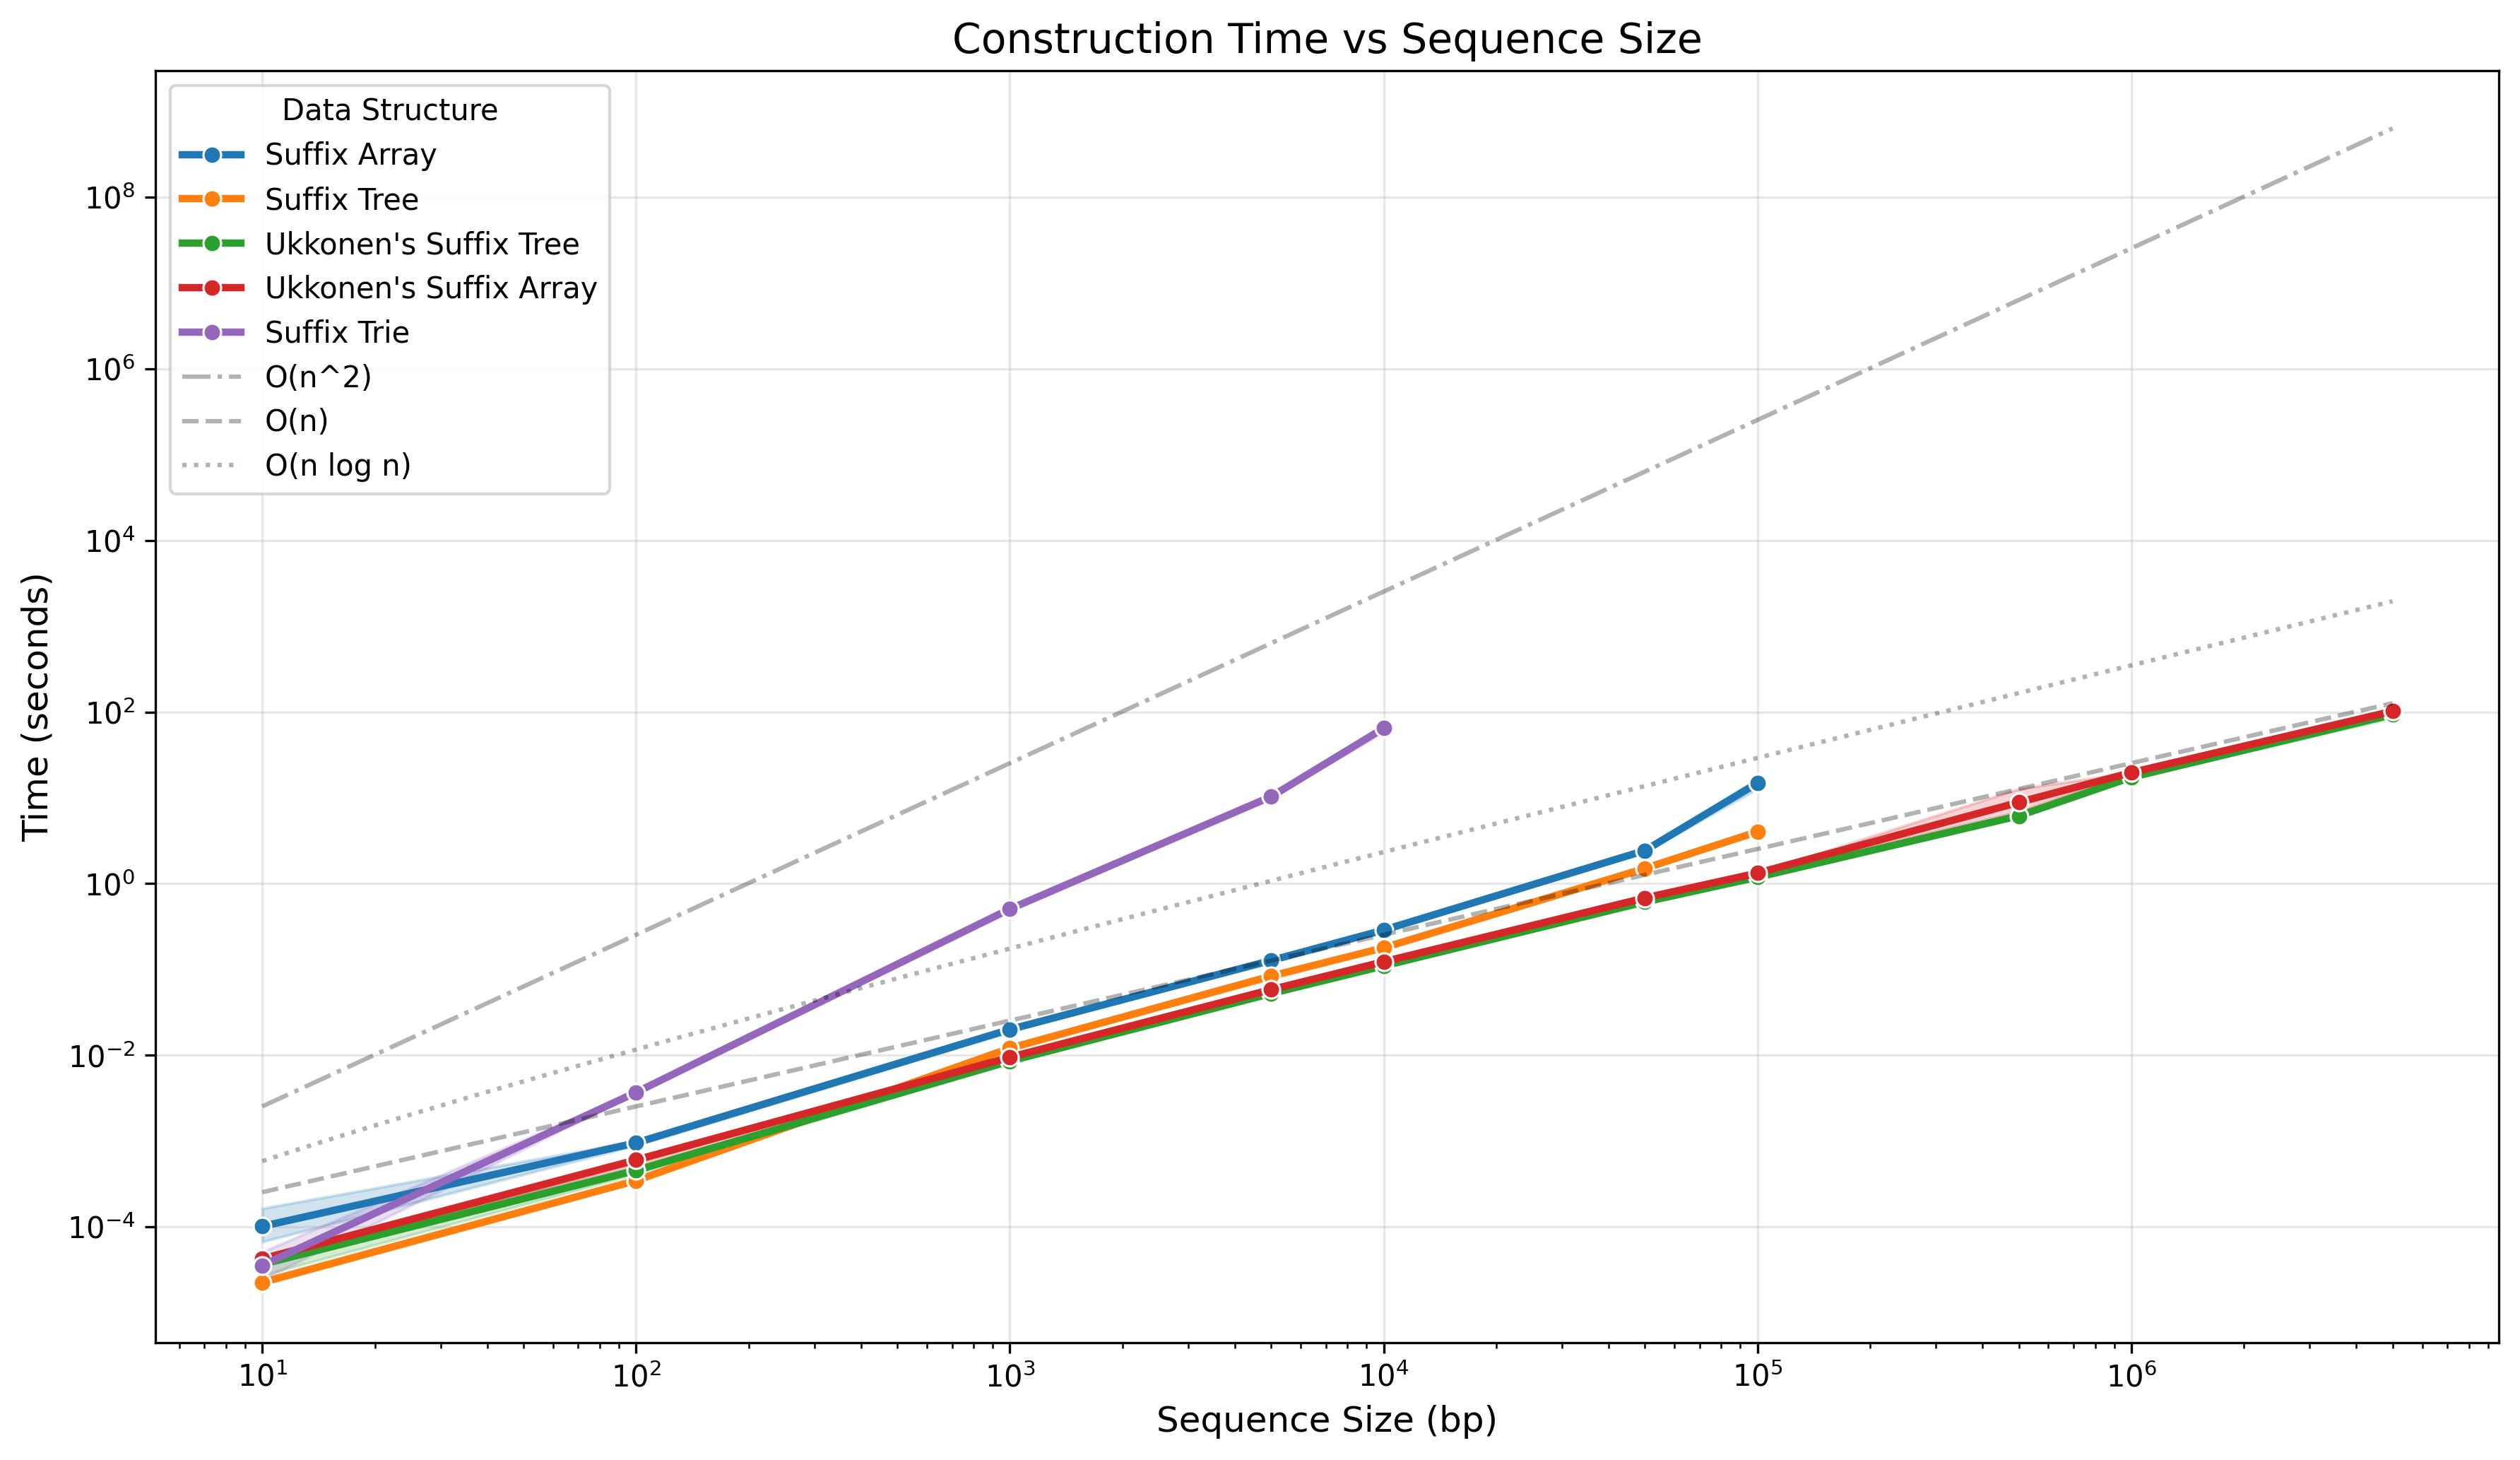
\includegraphics[width=0.6\textwidth]{../figures/construction_time.png}
  \caption{Runtime comparison of suffix tries, trees, and arrays for construction.}
  \label{fig:construction_time}
\end{figure}


Figure \ref{fig:construction_time} below displays a comparison of the runtime for constructing each of the suffix data structures, as it scales with the size of the input sequence.
The red and green lines representing Ukonnen's suffix tree and suffix array construction algorithms respectively, show the best scaling with the size of the input sequence.
The purple line represents the suffix trie, which is by far the slowest and most memory intensive to construct. My laptop ran out of memory when trying to construct a suffix trie for an input sequence larger than 10,000.
My gaming PC with significantly more available memory was able to run the computations at a higher level, but for practical purposes, the suffix trie is not a viable option for large input sequences.
It is clear that the suffix array constructed using Ukonnen's algorithm is the most efficient data structure in terms of construction time, and is the best choice for large input sequences,
while the suffix trie is the least efficient and should be avoided for large input sequences. \\

\begin{figure}[ht]
  \centering
  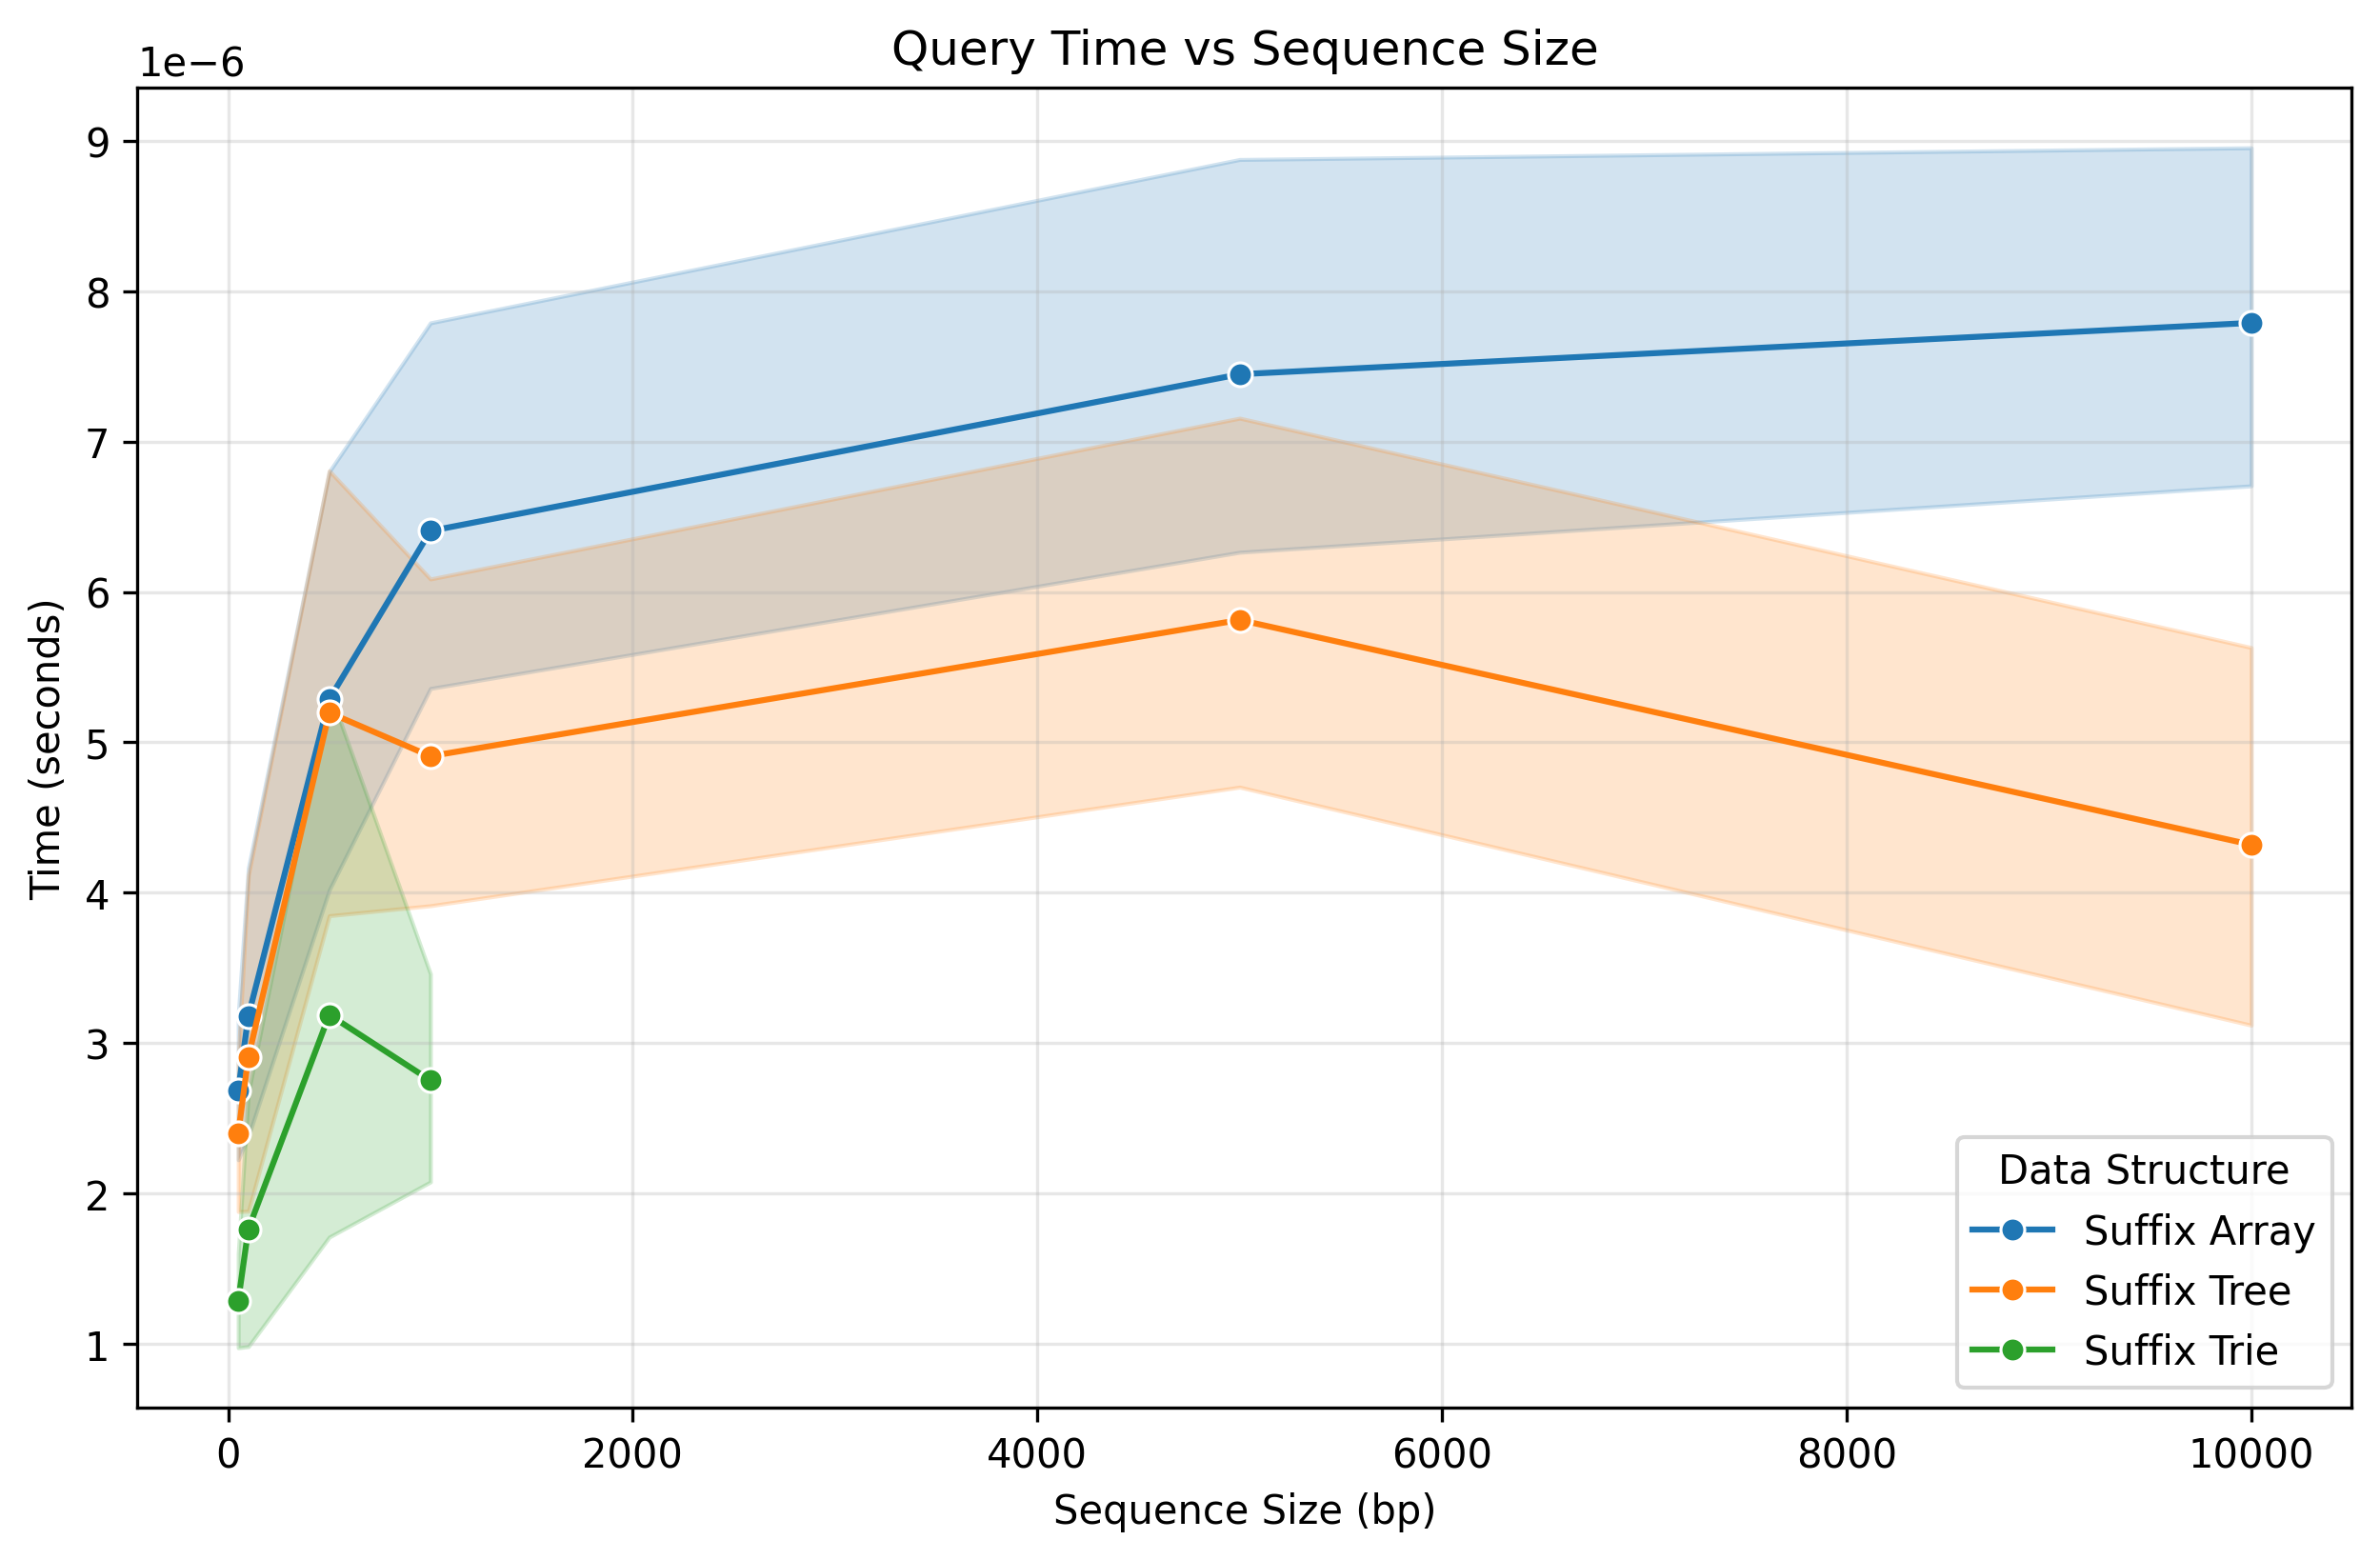
\includegraphics[width=0.6\textwidth]{../figures/query_time_by_size.png}
  \caption{Runtime comparison of suffix tries, trees, and arrays for querying.}
  \label{fig:query_time}
\end{figure}

Figure \ref{fig:query_time} below shows the runtime for querying each of the suffix data structures, as it scales with the size of the input sequence.
In this case, the suffix array constructed using Ukonnen's algorithm is the most efficient data structure for querying, followed by the suffix array constructed using the naive approach.
Its somewhat surprising that the suffix trie is more efficient here, but the graphs trend indicates that the suffix trie is likely to become less efficient if the input sequence size is increased,
while the suffix arrays seem to remain more stable at scale.

\subsection{Memory Usage Comparison}

Figure \ref{fig:memory_usage} shows the memory usage for constructing each of the suffix data structures, as it scales with the size of the input sequence.
This is the most interesting graph, with a very clear trend that the suffix trie is the most memory intensive, and Ukonnen's suffix array and tree being the least memory intensive.
As the size of the input sequence increases, the suffix trie becomes less and less viable, while Ukonnens suffix array and tree remain stable and efficient at scale, displaying a linear memory usage.
The suffix array constructed with the modified BFS approach is more memory intensive than Ukonnen's suffix array, but still significantly more efficient than the suffix trie.

\begin{figure}[ht]
  \centering
  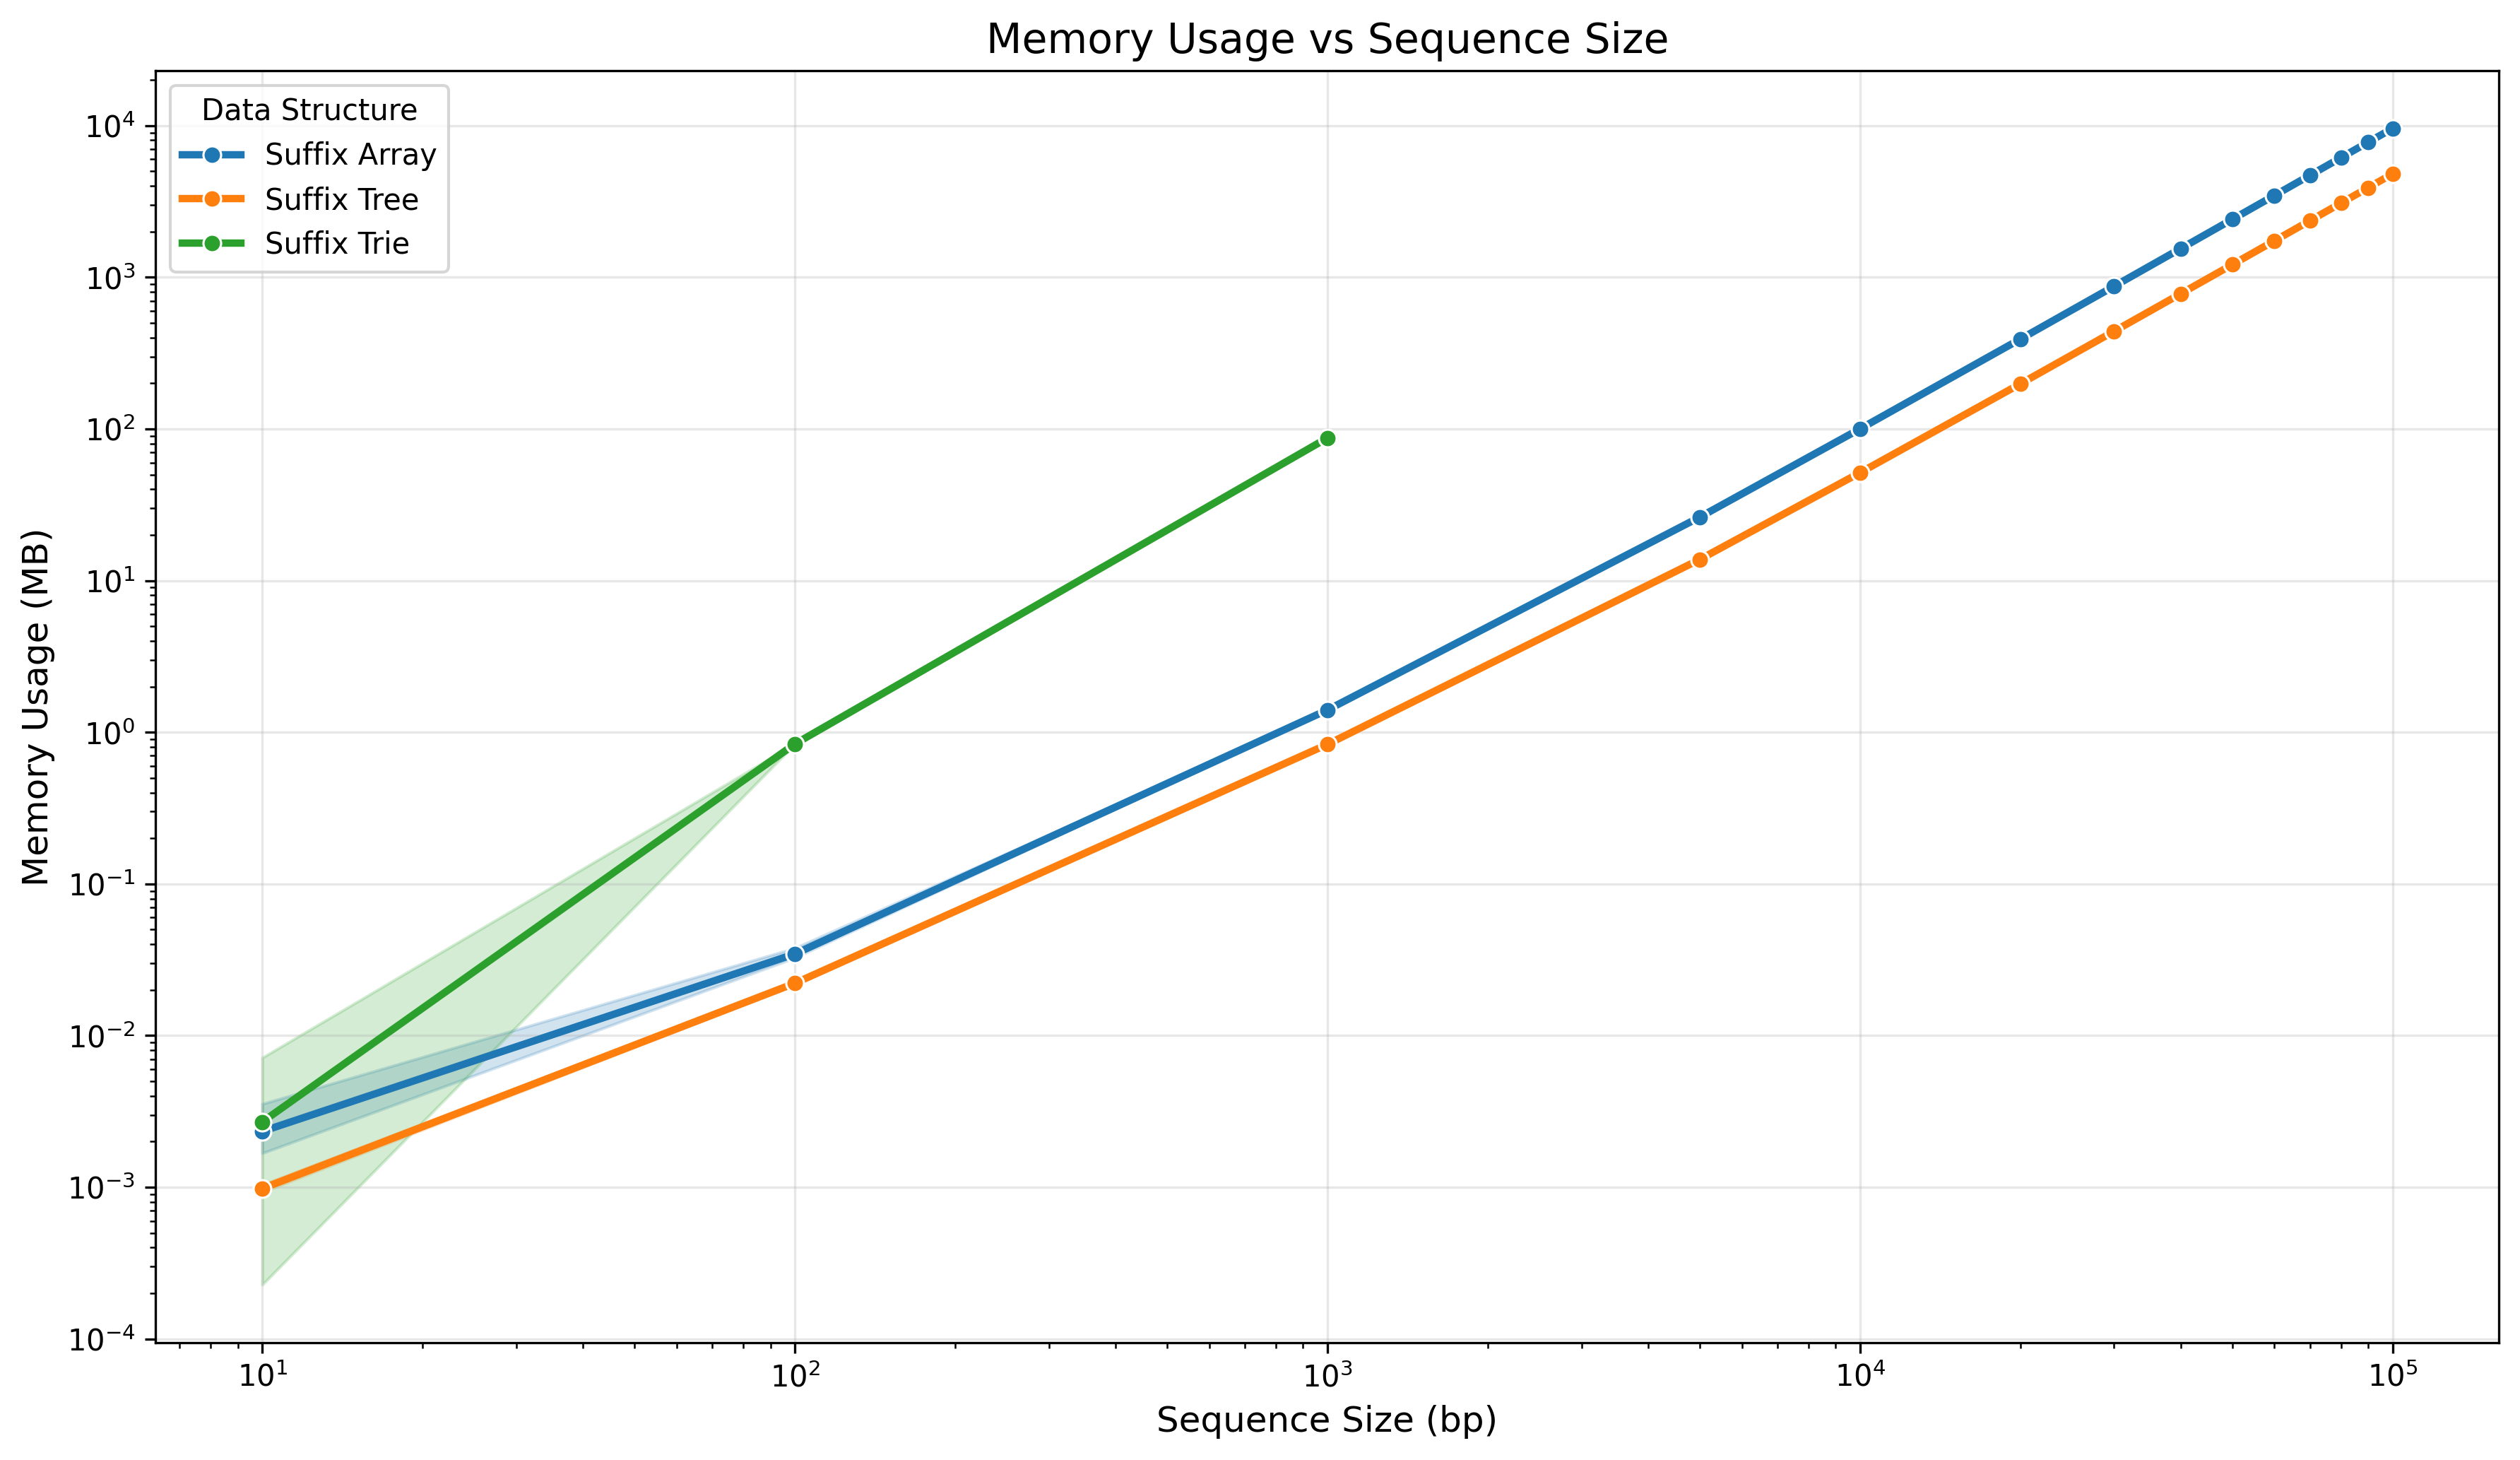
\includegraphics[width=0.6\textwidth]{../figures/memory_usage.png}
  \caption{Memory usage comparison of suffix tries, trees, and arrays for construction.}
  \label{fig:memory_usage}
\end{figure}

\section{Methods}

\subsection{}

\subsection{}

\subsection{}


\subsection{}

\section{Conclusion}

\section{Dependencies}
\begin{itemize}
  \item numpy
  \item subprocess
  \item psutil
  \item pandas
  \item seaborn
  \item matplotlib
  \item tqdm
  \item argparse
  \item gzip
  \item os 
  \item glob
  \item GraphicViz
\end{itemize}

\subsection{Installing GraphicViz}
To install GraphicViz, the package used to generate the trees and tries in this document, run the following command:
\begin{verbatim}
$ pip3 install git+https://github.com/cjdrake/ipython-magic.git
\end{verbatim}

\newpage

\section{Reproducibility}
\subsection{Commands to collect this data and reproduce the results}
I ran these commands to generate and collect the data for the figures in this report. \\
\textbf{NOTE:} You may need to install some dependencies specified in the README.md file and section 4 of this document. \\
\textbf{ALSO NOTE:} These commands are shell scripts that can take up to 30 minutes to run, 
depending on how fast your CPU is.
\begin{verbatim}
$ git clone https://github.com/cu-compg-spring-2025/assignment-6-suffix-index-JasonHunter95.git
$ cd assignment-6-suffix-index-JasonHunter95
$ python3 src/benchmark.py
\end{verbatim}

\subsection{Commands to run the suffix trie, tree, and array visualizations}
I ran these commands to generate the suffix trie, tree, and array visualizations in this document. \\
\textbf{NOTE:} You may need to install some dependencies specified in the README.md file and section 4 of this document. \
\begin{verbatim}
$ python3 src/suffix_trie.py \
--string BANANA \
--query ANANA NANA ANA A NA $ BANANA$
\end{verbatim}

\begin{verbatim}
$ python3 src/suffix_tree.py \
--string BANANA \
--query ANANA NANA ANA A NA $ BANANA$
\end{verbatim}

\begin{verbatim}
$ python3 src/suffix_array.py \
--string BANANA \
--query ANANA NANA ANA A NA $ BANANA$
\end{verbatim}

\subsection{Commands to visualize a region of a FASTA file for the suffix structures}
\begin{verbatim}
$ python3 src/suffix_trie.py \
--reference data/chr22.fa.gz \
--query ACGT \
--region 18800-18900
\end{verbatim}

\begin{verbatim}
$ python3 src/suffix_tree.py \
--reference data/chr22.fa.gz \
--query ACGT \
--region 18800-18900
\end{verbatim}

\begin{verbatim}
$ python3 src/suffix_array.py \
--reference data/chr22.fa.gz \
--query ACGT \
--region 18800-18900
\end{verbatim}

\begin{verbatim}
$ python3 src/ukonnens_suffix_tree.py \
--reference data/chr22.fa.gz \
--query ACGT \
--region 18800-18900
\end{verbatim}

\begin{verbatim}
$ python3 src/ukonnens_suffix_array.py \
--reference data/chr22.fa.gz \
--query ACGT \
--region 18800-18900
\end{verbatim}

To reproduce these, clone the repository, 
ensure that you are in the root directory and run the above commmands.
The data files are located in the data directory
and the scripts are located in the src directory
in the repository root.

\end{document}